\documentclass[12pt]{IEEEtran}

\usepackage[brazilian]{babel}
\usepackage[utf8]{inputenc}
\usepackage{amsmath}
\usepackage{mathtools}
\usepackage{indentfirst}
\usepackage{graphicx}
\usepackage{multicol,lipsum}
\usepackage{float}
\usepackage{steinmetz}
\usepackage{adjustbox}


\title{Relatório Experimental 1 - Prática de Física dos Dispositivos Eletrônicos}
\author{Felipe Rodrigues Sobrinho (17/0141764)}
\date{14/06/2022}




\begin{document}

\maketitle

\section{Introdução}

A resistividade é uma das características dos circuitos elétricos mais simples e com certeza a mais difundida. 
Tal lei é determinada, basicamente, pela oposição de uma estrutura a passagem de elétrons, transformando 
o excedente em calor. 

Esse trabalho tem o objetivo de observar a resistividade do grafite em uma folha. A partir dos dados
obtidos experimentalmente e dos conhecimentos teóricos, tentar-se-á desenvolver as características 
da camada do grafite, como a espessura.


\section{Metodologia}

Para tal experimento, foi utilizado a bancada experimental vista na figura \ref{fig:bancada}. Foi utilizado um multímetro do modelo DT9205A e uma fonte de bancada do modelo POL-16E.

\begin{figure}[H]
  \centering
  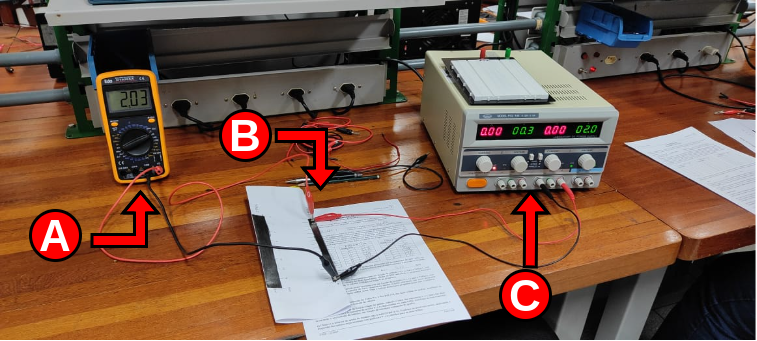
\includegraphics[width=.48\textwidth]{bancada_imagem.png}
  \caption{Bancada experimental utilizada. A) Multímetro XXXX; B) Folha com as trilhas de grafite preenchidas; C) Fonte de alimentação POL-16E.}
  \label{fig:bancada}
\end{figure}



O primeiro experimento envolve a medição de tensão sobre a trilha resistiva construída. Tal medição foi feita como visto na figura \ref{fig:medicao_tensao}.

\begin{figure}[H]
  \centering
  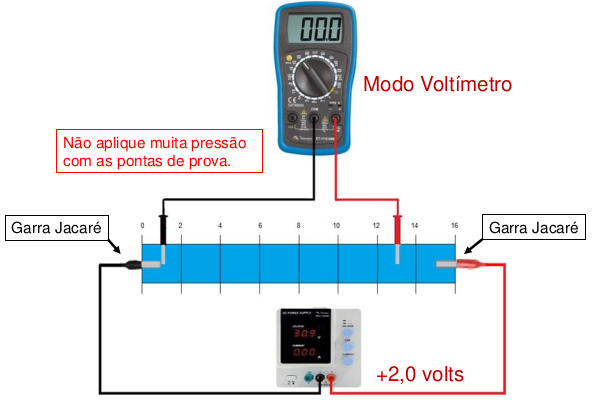
\includegraphics[width=.48\textwidth]{medicao_tensao.png}
  \caption{Método para medição da variação de tensão sobre a superfície da folha.}
  \label{fig:medicao_tensao}
\end{figure}



O segundo experimento conta com a medição da resistência efetiva da trilha construída, cujo método de medição pode ser visto na figura \ref{fig:medicao_resistencia}.

\begin{figure}[H]
  \centering
  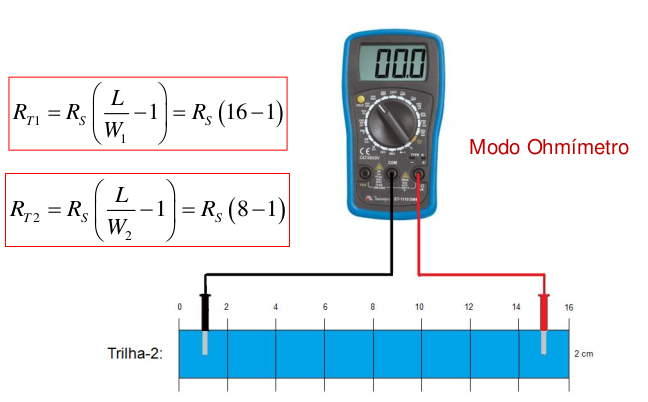
\includegraphics[width=.48\textwidth]{medicao_resistencia.png}
  \caption{Método para medição da resistência total da camada de grafite.}
  \label{fig:medicao_resistencia}
\end{figure}




\section{Resultados}

\subsection{Variação de tensão sobre a trilha}

Para verificar a tensão sobre a trilha, foi utilizado o método visto na figura . Com isso, foi possível, para ambas as trilhas, criar as tabelas \ref{tab:trilha_1} e \ref{tab:trilha_2}, que compreendem as tensões nos pontos equidistantes das trilhas.

\begin{table}[H]
\centering
\caption{Relação entre tensão mensurada em cada quadrado da trilha 1.}
\label{tab:trilha_1}
\begin{tabular}{cccc}
\hline
\multicolumn{4}{c}{\textbf{Trilha-1: W = 1 cm}}                                      \\ \hline
\textbf{Quadrado} & \multicolumn{1}{c|}{\textbf{Vi}} & \textbf{Quadrado} & \textbf{Vi} \\ \hline
1                 & \multicolumn{1}{c|}{0}           & 9                 & 1,040       \\ \hline
2                 & \multicolumn{1}{c|}{0,201}       & 10                & 1,170       \\ \hline
3                 & \multicolumn{1}{c|}{0,314}       & 11                & 1,273       \\ \hline
4                 & \multicolumn{1}{c|}{0,429}       & 12                & 1,385       \\ \hline
5                 & \multicolumn{1}{c|}{0,544}       & 13                & 1,501       \\ \hline
6                 & \multicolumn{1}{c|}{0,641}       & 14                & 1,668       \\ \hline
7                 & \multicolumn{1}{c|}{0,770}       & 15                & 1,855       \\ \hline
8                 & \multicolumn{1}{c|}{0,899}       & 16                & 2,03        \\ \hline
\end{tabular}
\end{table}



\begin{table}[H]
\centering
\caption{Relação entre tensão mensurada em cada quadrado da trilha 2.}
\label{tab:trilha_2}
\begin{tabular}{cc}
\hline
\multicolumn{2}{c}{\textbf{Trilha-2: W = 2 cm}} \\ \hline
\textbf{Quadrado}         & \textbf{Vi}         \\ \hline
1                         & 0                   \\ \hline
2                         & 0,405               \\ \hline
3                         & 0,711               \\ \hline
4                         & 1,058               \\ \hline
5                         & 1,396               \\ \hline
6                         & 1,618               \\ \hline
7                         & 1,805               \\ \hline
8                         & 1,97                \\ \hline
\end{tabular}
\end{table}

\subsection{Resistência efetiva da trilha}

Para calcular a resistência efetiva da trilha, foi utilizado o método visto na figura xxx. Assim, para a trilha de 1cm a resistência medida foi de $12,58k\Omega$ e para a trilha de 2cm a resitência medida foi de $9,48k\Omega$. 


\subsection{Ajuste do modelo linear}

Nas figuras \ref{fig:adjust_trilha_1} e \ref{fig:adjust_trilha_2}, é possível ver os gráficos de um modelo linear com base nos pontos obtidos na tabela \ref{tab:trilha_1} e \ref{tab:trilha_2}, respectivamente. Em cada gráfico, também está disposto o valor do erro quadrático médio associado.

\begin{figure}[H]
  \centering
  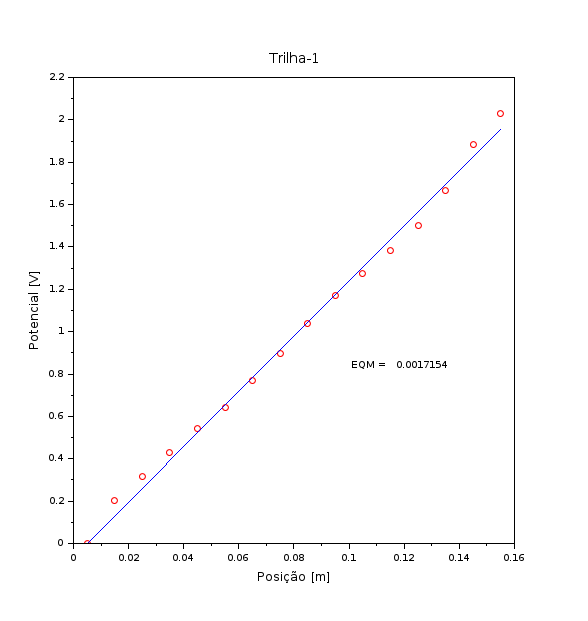
\includegraphics[width=.48\textwidth]{curva_ajustada_trilha_1.png}
  \caption{Ajuste do modelo linear e erro quadrático médio dos pontos da trilha 1.}
  \label{fig:adjust_trilha_1}
\end{figure}

\begin{figure}[H]
  \centering
  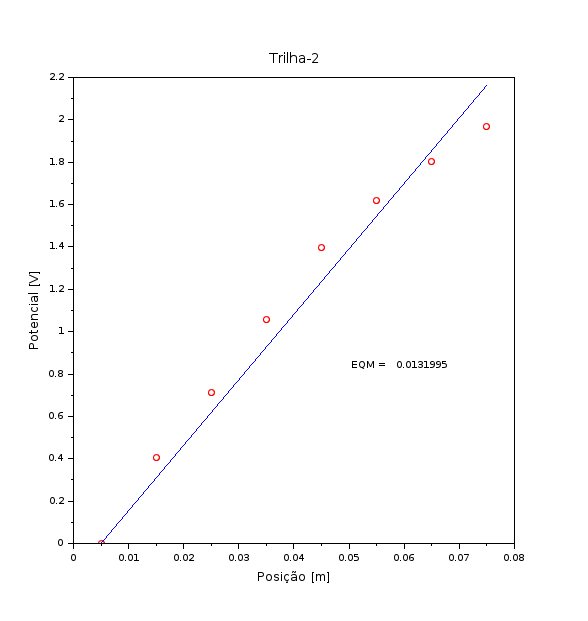
\includegraphics[width=.48\textwidth]{curva_ajustada_trilha_2.png}
  \caption{Ajuste do modelo linear e erro quadrático médio dos pontos da trilha 2.}
  \label{fig:adjust_trilha_2}
\end{figure}

\section{Questionário}

\subsection{Calcule os valores das Resistências de folha Rs1 e Rs2 [$k\Omega/quadrado$] das duas trilhas de grafite. Justifique as suas respostas, mostrando o seu método de cálculo.}

Temos que a resistividade do grafite é dada por $\rho=7,8\times 10^{-6}[\Omega \cdot m]$. Assim, obtemos o valor de Rs1 a partir da equação \ref{Rs1_val}.

\begin{gather}\label{Rs1_val}
  Rs1 = \dfrac{R_{T1}}{(16-1)} 
\end{gather}

Assim, o valor de $Rs1$ é $838,67$. Nesse mesmo sentido, temos que o valor de $Rs2$ será dado pela equação \ref{Rs2_val}.

\begin{gather}\label{Rs2_val}
  Rs2 = \dfrac{R_{T2}}{(8-1)} 
\end{gather}

O valor de $Rs2$ é $1354.28$. Tais resultados são razoáveis.



\subsection{A partir do valor de tabela da Resistividade do grafite, calcule o valor de espessura t1 e t2 [nm] das duas trilhas. Estime o número de camadas de grafite n1 e n2 depositadas em cada trilha. Justifique suas respostas, mostrando o método de cálculo, em função da estrutura conhecida do grafite.}

A espessura dos grafites pode ser dada pela equação \ref{t}.

\begin{gather}\label{t}
  t = \dfrac{\rho}{Rs} 
\end{gather}

Logo, as espessuras t1 e t2 serão, respectivamente, $9,3\times 10^{-9}$ e $5,75\times 10^{-9}$.

Tais valores de t1 e t2 correspondem, respectivamente, a $9,3$ camadas de grafite e $5,75$ camadas de grafite.


\subsection{Observe a métrica de ajuste do modelo não é nula ($EQM\neq 0$). Explique as possíveis razões, analisando a dispersão dos pontoos experimentais nos gráficos ($V_i \times x_i$) obtidos para as duas trilhas.}

O valor de erro é não nulo por uma série de fatores externos incontroláveis que perturbam a experimentação e, consequentemente, afetam os resultados. Alguns desses elementos são:

\begin{itemize}
  \item Variação na tensão da fonte de alimentação;
  \item Não medição nos centros dos quadrados;
  \item Imprecisão imposta por meio das pontas de prova;
  \item Imprecisão do multímetro;
  \item Não uniformidade da camada de grafite (esse é um fator muito importante);
  \item Não uniformidade no formato da camada de grafite;
\end{itemize}





\end{document}
